\documentclass[openany]{book}
\usepackage[utf8]{inputenc}
\usepackage{graphicx}
\usepackage{caption}
\usepackage{minted}
\usepackage[spanish]{babel}

\usepackage{multicol}
\usepackage{multirow}
\usepackage[T1]{fontenc}
\usepackage{changepage}
\usepackage{float}
\usepackage{url}
\usepackage[table,xcdraw]{xcolor}
\usepackage[left=2.5cm,right=2.5cm,top=2.5cm,bottom=2.5cm]{geometry}
\usepackage{parskip}
\usepackage{blindtext}
\usepackage{multicol}
\usepackage{wrapfig}
\usepackage{subcaption}

\usepackage{enumitem}
\usepackage{hyperref}
\hypersetup
{
    colorlinks=true,
    linkcolor=blue,
    filecolor=magenta,      
    urlcolor=cyan,
    pdftitle={Sitio Web del Laboratorio de Instrumentación Electrónica de Sistemas Espaciales},
    pdfauthor={LIESE},
    pdfsubject={Sitio Web del Laboratorio de Instrumentación Electrónica de Sistemas Espaciales},
    pdfkeywords={Django, Python, HTML, CSS, JavaScript, Bootstrap, PostgreSQL, Nginx, Gunicorn, Ubuntu Server, SSH, Systemd},
    pdfpagemode=FullScreen,
}

% Tablas
\usepackage{array, multirow, multicol}
\usepackage{multirow}
%\usepackage[table,xcdraw]{xcolor}
\usepackage{longtable,tabu}
\usepackage[online]{threeparttablex}
\usepackage{cite} % Better handling of numeric citations

% Center without space
\newenvironment{nscenter}
{\parskip=0pt\par\nopagebreak\centering}
{\par\noindent\ignorespacesafterend}

\newcolumntype{M}[1]{>{\centering\arraybackslash}m{#1}}
\newcolumntype{C}[1]{>{\centering\arraybackslash}m{#1}}

\usepackage{tabularx}
\usepackage{lipsum}
\usepackage{ltablex}



\definecolor{mGreen}{rgb}{0,0.6,0}
\definecolor{mGray}{rgb}{0.5,0.5,0.5}
\definecolor{mPurple}{rgb}{0.58,0,0.82}
\definecolor{backgroundColour}{rgb}{0.95,0.95,0.92}

\usepackage{color, colortbl}
\definecolor{LightCyan}{rgb}{0.88,1,1}

\usepackage[first=0,last=9]{lcg}
\newcommand{\ra}{\rand0.\arabic{rand}}

\newenvironment{Figura}
  {\par\medskip\noindent\minipage{\linewidth}}
  {\endminipage\par\medskip}

\let\origdoublepage\cleardoublepage
\renewcommand{\cleardoublepage}{\clearpage}

\renewcommand{\bibname}{Referencias}

\title{SITIO WEB DEL LABORATORIO DE INSTRUMENTACIÓN ELECTRÓNICA DE SISTEMAS ESPACIALES}
\author{LIESE}
\date{\today}

\begin{document}
  \begin{titlepage}
  \thispagestyle{empty}
  \begin{minipage}[c][0.17\textheight][c]{0.25\textwidth}
    \begin{center}
    \hspace*{-15mm}
      
\includegraphics[height=4.5cm]{Imagenes/escudounam_negro.jpg}
    \end{center}
  \end{minipage}
  \begin{minipage}[c][0.195\textheight][t]{0.75\textwidth}
    \begin{center}
      \vspace{0.3cm}
             {\color{black}\textsc{\huge Universidad Nacional Autónoma de México} }\\[1cm]
          
                    {\color{black}\hrule height2pt}
                    \vspace{.2cm}
                           {\color{black}\hrule height1pt}
                           \vspace{1.5cm}
                           \textsc{\LARGE Facultad de Ingeniería\\ División Ingeniería Eléctrica}
    \end{center}
  \end{minipage}
  \begin{minipage}[c][0.81\textheight][t]{0.25\textwidth}
    \vspace*{5mm}
    \begin{center}
      \hskip0.5mm
             \vspace{5mm}
             \hskip2pt
                 {\color{black}\vrule width3pt height13cm}
                 \hskip2mm
                     {\color{black}\vrule width1pt height13cm} \\
                     \vspace{5mm}
                     \hspace*{-15mm}
             
\includegraphics[height=5cm]{Imagenes/escudofi_negro.jpg}
    \end{center}
  \end{minipage}
  \begin{minipage}[c][0.81\textheight][t]{0.75\textwidth}
    \begin{center}
      \vspace{2cm}

      {\color{black}{\LARGE \scshape Laboratorio de Instrumentación Electrónica de Sistemas Espaciales}\\[.2in]
      \vspace{4 cm}            
{\color{black}\hrule height1pt}
\vspace{0.25 cm}  
\begin{center}
\LARGE \scshape SITIO WEB DEL LABORATORIO DE INSTRUMENTACIÓN ELECTRÓNICA DE SISTEMAS ESPACIALES
\vspace{0.25 cm}  
{\color{black}\hrule height1pt}
\vspace{3 cm}
\end{center}

 }

    \end{center}
  \end{minipage}
\end{titlepage}
%---------------------------------
  \maketitle
  \tableofcontents
  \newpage
  \chapter{Introducción}

\section{Presentación del LIESE}
El Laboratorio de Instrumentación Electrónica de Sistemas Espaciales (LIESE) es una unidad académica adscrita a la División de Ingeniería Eléctrica de la Facultad de Ingeniería de la Universidad Nacional Autónoma de México (UNAM). Su misión es impulsar la formación de especialistas y el desarrollo de tecnología en el área espacial, con énfasis en el diseño, construcción e implementación de sistemas electrónicos para aplicaciones satelitales, instrumentación embebida, Internet de las Cosas (IoT) e inteligencia artificial. El LIESE promueve la colaboración interdisciplinaria y la innovación tecnológica, contribuyendo al avance científico y al bienestar social en México.

\section{Objetivos del sitio web}
El sitio web del LIESE tiene como objetivos principales:
\begin{itemize}
    \item Difundir los proyectos, logros y actividades del laboratorio a la comunidad académica y al público en general.
    \item Facilitar el reclutamiento de nuevos talentos y la vinculación con otras instituciones.
    \item Proveer un canal de comunicación actualizado sobre eventos, oportunidades y noticias relevantes.
    \item Servir como plataforma de gestión y administración de contenido para los miembros del laboratorio.
\end{itemize}

\section{Alcance del sistema web}
El sistema web desarrollado abarca las siguientes funcionalidades:
\begin{itemize}
    \item Publicación y gestión de artículos, tesis y noticias.
    \item Visualización de proyectos y actividades del laboratorio.
    \item Calendario de eventos académicos y de divulgación.
    \item Sección de líderes de proyecto y miembros del laboratorio.
    \item Sistema de oportunidades con autenticación de dos factores (2FA) para solicitudes.
    \item Panel de administración basado en Django para la gestión de contenido.
    \item Interfaz responsiva y moderna, accesible desde dispositivos móviles y de escritorio.
\end{itemize}

\section{Justificación del desarrollo}
El desarrollo de un sitio web institucional es fundamental para fortalecer la presencia digital del LIESE, facilitar la comunicación interna y externa, y promover la transparencia y el acceso a la información. La plataforma permite centralizar la gestión de contenido, automatizar procesos administrativos y ofrecer una experiencia de usuario moderna y segura. Además, la integración de mecanismos de seguridad como la verificación por correo electrónico y la autenticación de dos factores contribuye a la protección de los datos y la confianza de los usuarios.

  \chapter{Marco Teórico y Conceptual}

\section{Django Framework}
Django es un framework de desarrollo web de alto nivel, escrito en Python, que fomenta el desarrollo rápido y limpio de aplicaciones web. Utiliza el patrón arquitectónico Modelo-Vista-Template (MVT), el cual separa la lógica de negocio, la presentación y el acceso a datos, facilitando la mantenibilidad y escalabilidad del sistema \cite{django-docs}. Django incluye un sistema de administración automática, un ORM (Object-Relational Mapping) para interactuar con bases de datos, y herramientas integradas para la gestión de usuarios, seguridad y envío de correos electrónicos. Entre sus características destacan la protección contra ataques comunes (CSRF, XSS, SQL Injection), el sistema de migraciones para la evolución del esquema de datos y la posibilidad de extender la funcionalidad mediante aplicaciones reutilizables. Es ampliamente utilizado en la industria y en el ámbito académico por su robustez, flexibilidad y comunidad activa.

El patrón MVT de Django se compone de:
\begin{itemize}
    \item \textbf{Modelo}: Define la estructura de los datos y su representación en la base de datos.
    \item \textbf{Vista}: Gestiona la lógica de negocio y responde a las solicitudes del usuario.
    \item \textbf{Template}: Controla la presentación y el renderizado de la información al usuario final.
\end{itemize}

\section{Tecnologías Frontend}
El frontend del sitio web está construido utilizando HTML5, CSS3 y el framework Bootstrap 5.3.3. HTML5 proporciona la estructura semántica de las páginas, permitiendo una mejor accesibilidad y posicionamiento en buscadores. CSS3 permite el diseño visual, la adaptación responsiva a diferentes dispositivos y la implementación de animaciones y transiciones. Bootstrap es una biblioteca de componentes y utilidades CSS/JS que facilita la creación de interfaces modernas, responsivas y accesibles, acelerando el desarrollo y asegurando la compatibilidad multiplataforma \cite{bootstrap-docs}. Se emplean también animaciones CSS y JavaScript para mejorar la experiencia de usuario, así como la integración de iconos y recursos multimedia.

\section{Base de Datos}
Durante el desarrollo, el sistema utiliza SQLite como base de datos por su simplicidad y portabilidad. SQLite es una base de datos relacional embebida, ideal para entornos de desarrollo y pruebas. Para entornos de producción, se recomienda el uso de PostgreSQL, un sistema de gestión de bases de datos relacional robusto, escalable y con soporte avanzado para transacciones, concurrencia y extensiones \cite{postgresql-docs}. Django abstrae el acceso a la base de datos mediante su ORM, permitiendo definir modelos de datos en Python y realizar migraciones automáticas. Esto facilita la evolución del esquema de datos y la portabilidad entre diferentes motores de base de datos. El uso de migraciones garantiza la integridad y consistencia de los datos a lo largo del ciclo de vida del proyecto.

\section{Servicios Web}
El sitio web implementa servicios de correo electrónico para la verificación de usuarios y la autenticación de dos factores (2FA) en el sistema de oportunidades. Utiliza el protocolo SMTP para el envío de correos, configurado en el archivo de settings de Django \cite{django-email}. Además, el sistema aprovecha las capacidades de seguridad integradas de Django, como la protección contra CSRF, la gestión de sesiones y la validación de formularios. El uso de formularios seguros y la validación del lado del servidor son fundamentales para prevenir ataques y garantizar la integridad de la información.

\section{Despliegue}
El despliegue del sistema se realiza sobre servidores Ubuntu, un sistema operativo de código abierto ampliamente utilizado en entornos de servidores por su estabilidad, seguridad y soporte a largo plazo (LTS) \cite{ubuntu-docs}. El servicio se gestiona mediante Systemd, utilizando el comando \texttt{runserver} de Django para exponer la aplicación en la red local, de acuerdo con el archivo de unidad real utilizado en el proyecto. El servicio se ejecuta bajo un usuario específico, define el directorio de trabajo y reinicia automáticamente en caso de fallo. Los archivos estáticos y media se sirven mediante la configuración de Django. Aunque en entornos de producción se recomienda el uso de Gunicorn y Nginx para mayor robustez y rendimiento, en este despliegue se utiliza el servidor de desarrollo de Django para simplificar la administración. El proceso de despliegue incluye la migración de la base de datos y la recolección de archivos estáticos, siguiendo buenas prácticas de administración de servicios en Linux.

  \chapter{Análisis y Requerimientos}
\section{Requerimientos Funcionales}
Los requerimientos funcionales describen las capacidades y servicios que el sistema debe proporcionar a los usuarios finales. Para el sitio web del Laboratorio de Instrumentación Electrónica de Sistemas Espaciales (LIESE), se identifican los siguientes:
\begin{itemize}
	\item Registro y gestión de miembros del laboratorio, incluyendo líderes de proyecto y administradores.
	\item Visualización de información sobre proyectos, artículos, eventos y noticias.
	\item Solicitud de oportunidades académicas (investigación, tesis, maestría, servicio social) mediante formularios web y verificación de correo electrónico.
	\item Publicación y administración de artículos, eventos y noticias por parte de usuarios autorizados.
	\item Sistema de autenticación y autorización para acceso a panel de administración y funcionalidades restringidas.
	\item Envío de correos electrónicos automáticos para verificación y notificaciones relevantes.
	\item Gestión de archivos multimedia (imágenes, documentos) asociados a miembros, proyectos y artículos.
	\item Interfaz de usuario responsiva y accesible para diferentes dispositivos.
\end{itemize}
\section{Requerimientos No Funcionales}
Los requerimientos no funcionales establecen criterios de calidad, restricciones y condiciones bajo las cuales el sistema debe operar:
\begin{itemize}
	\item Seguridad: Protección contra ataques comunes (CSRF, XSS, SQL Injection) y gestión segura de sesiones y contraseñas \cite{django-docs}.
	\item Rendimiento: Respuesta eficiente a las solicitudes de los usuarios y manejo adecuado de archivos estáticos y multimedia.
	\item Escalabilidad: Capacidad de migrar de SQLite a PostgreSQL para soportar mayor volumen de datos y usuarios \cite{postgresql-docs}.
	\item Mantenibilidad: Código estructurado siguiendo el patrón MVT de Django y uso de migraciones para la evolución del esquema de datos.
	\item Disponibilidad: Despliegue en servidores Ubuntu con servicios gestionados por Systemd y balanceo de carga mediante Nginx \cite{ubuntu-docs,nginx-docs}.
	\item Accesibilidad: Cumplimiento de estándares web y diseño responsivo con Bootstrap \cite{bootstrap-docs}.
	\item Usabilidad: Interfaz intuitiva y documentación clara para usuarios y administradores.
\end{itemize}
\section{Casos de Uso}
Los casos de uso describen las interacciones principales entre los usuarios y el sistema. A continuación se presentan los casos de uso más relevantes:

\begin{itemize}
	\item \textbf{Registro de oportunidad académica:} Un visitante completa el formulario de solicitud, recibe un correo de verificación y, tras confirmar su correo, su solicitud es registrada y notificada a los administradores.
	\item \textbf{Gestión de miembros:} Un administrador agrega, edita o elimina miembros y líderes de proyecto desde el panel de administración.
	\item \textbf{Publicación de artículos y eventos:} Usuarios autorizados crean y editan artículos, eventos y noticias, incluyendo la carga de imágenes y documentos.
	\item \textbf{Visualización de información:} Cualquier usuario puede consultar información pública sobre proyectos, artículos, eventos y miembros del laboratorio.
	\item \textbf{Autenticación y acceso:} Los administradores y editores acceden a funcionalidades restringidas mediante autenticación segura.
\end{itemize}

  \chapter{Diseño y Arquitectura}
\section{Arquitectura MVT de Django}
El sistema está construido siguiendo el patrón Modelo-Vista-Template (MVT) de Django, que separa la lógica de negocio, la presentación y el acceso a datos \cite{django-docs}. Esta arquitectura facilita la mantenibilidad, escalabilidad y reutilización de componentes. El modelo representa la estructura y reglas de los datos, la vista gestiona la lógica de negocio y las respuestas a las solicitudes del usuario, y el template define la presentación visual de la información.

\begin{figure}[H]
	\centering
	% Diagrama UML de la arquitectura general (PlantUML)
	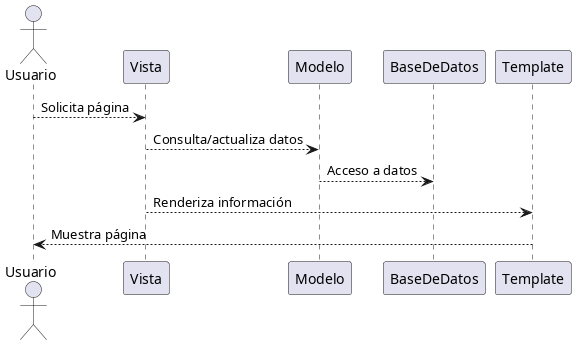
\includegraphics[width=0.8\textwidth]{uml/arquitectura-mvt.png}
	\caption{Diagrama UML de la arquitectura MVT de Django para el sitio LIESE.}
\end{figure}
\newpage
\section{Modelos de Datos}
El modelo de datos del sitio LIESE incluye entidades como Miembro, Proyecto, Artículo, Evento, Noticia y Solicitud de Oportunidad. Cada entidad se implementa como una clase en Django, con atributos que representan los campos de la base de datos y relaciones entre modelos (por ejemplo, un artículo tiene un autor que es un miembro, y un proyecto puede tener varios miembros asociados). El uso del ORM de Django permite definir, consultar y migrar los modelos de manera eficiente y segura.

\begin{figure}[H]
	\centering
	% Diagrama UML de clases de los modelos principales (PlantUML)
	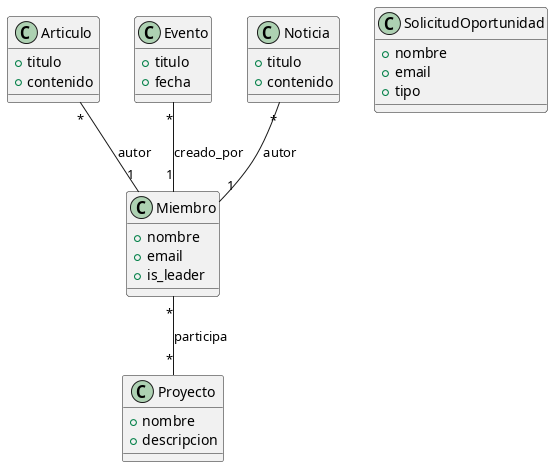
\includegraphics[width=0.95\textwidth]{uml/modelos-datos.png}
	\caption{Diagrama UML de clases de los modelos principales del sistema LIESE.}
\end{figure}
\newpage
\section{Diseño de Base de Datos}
La base de datos se diseña para soportar la gestión de información académica y administrativa del laboratorio. Se emplea SQLite en desarrollo y PostgreSQL en producción, aprovechando la portabilidad y robustez de ambos motores \cite{postgresql-docs}. Las migraciones de Django permiten evolucionar el esquema de datos sin pérdida de información. El diseño contempla claves foráneas para mantener la integridad referencial y relaciones muchos a muchos (por ejemplo, miembros y proyectos).

\begin{figure}[H]
	\centering
	% Diagrama UML entidad-relación simplificado (PlantUML)
	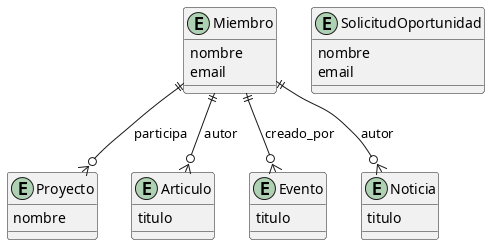
\includegraphics[width=0.95\textwidth]{uml/diagrama-er.png}
	\caption{Diagrama entidad-relación (ER) simplificado de la base de datos.}
\end{figure}
\section{Arquitectura de Templates}
La presentación del sitio se implementa mediante el sistema de templates de Django, que permite separar la lógica de presentación del código Python. Se utilizan plantillas HTML con etiquetas y filtros de Django para renderizar información dinámica, y se heredan estructuras comunes como la barra de navegación y el pie de página. El uso de Bootstrap facilita el diseño responsivo y accesible \cite{bootstrap-docs}.

\begin{figure}[H]
	\centering
	% Diagrama UML de herencia de templates (PlantUML)
	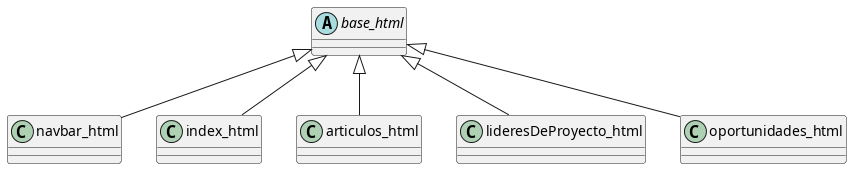
\includegraphics[width=0.7\textwidth]{uml/templates-herencia.png}
	\caption{Diagrama de herencia de templates en el sistema LIESE.}
\end{figure}

  \chapter{Implementación}
\section{Estructura del Proyecto Django}
La estructura del proyecto sigue la convención estándar de Django, separando la configuración, la aplicación principal y los recursos estáticos y de plantillas. A continuación se muestra un diagrama UML de la organización de carpetas y archivos principales:
\begin{figure}[H]
	\centering
	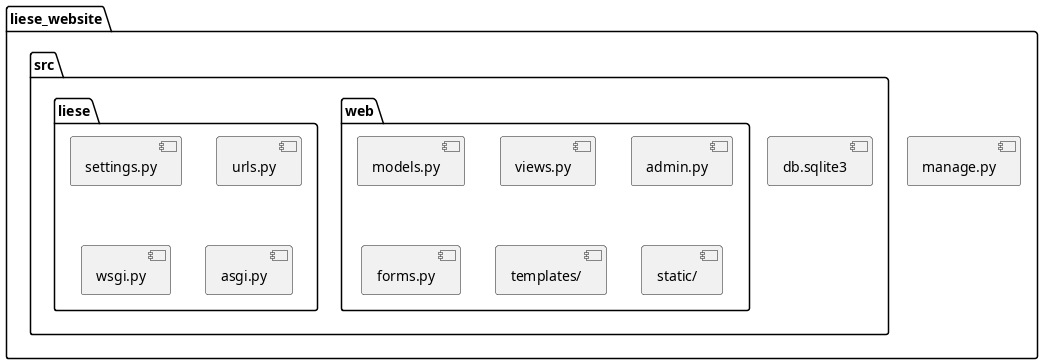
\includegraphics[width=0.9\textwidth]{uml/estructura-proyecto.png}
	\caption{Estructura de carpetas y archivos principales del proyecto Django LIESE.}
\end{figure}
\newpage
\section{Modelos, Vistas y URLs}
El flujo de interacción entre usuario, vistas y modelos se ilustra en el siguiente diagrama UML de secuencia, usando como ejemplo el proceso de solicitud de oportunidad académica:
\begin{figure}[H]
	\centering
	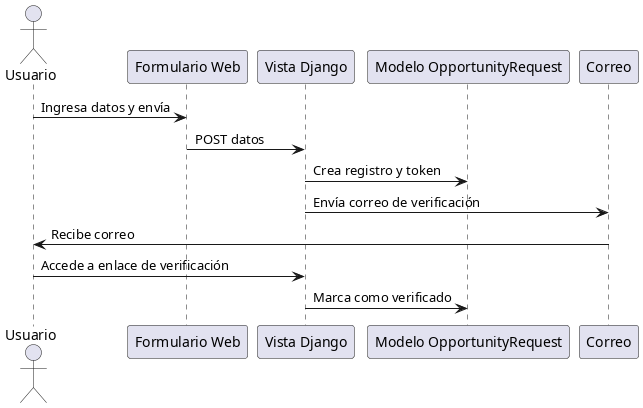
\includegraphics[width=0.95\textwidth]{uml/flujo-oportunidad.png}
	\caption{Diagrama de secuencia UML para el flujo de solicitud de oportunidad.}
\end{figure}
\section{Templates y Frontend}
El frontend utiliza el sistema de templates de Django y Bootstrap para la presentación. La herencia de plantillas y la organización de los archivos HTML ya se ilustró en el capítulo de arquitectura.
\newpage
\section{Sistema de Administración}
El panel de administración de Django permite gestionar usuarios, miembros, proyectos y contenidos. El siguiente diagrama UML de colaboración muestra la interacción entre el administrador, el panel y los modelos:
\begin{figure}[H]
	\centering
	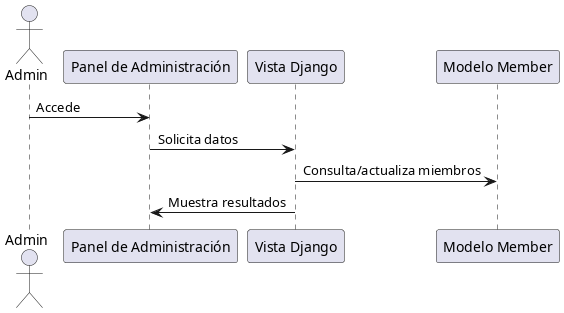
\includegraphics[width=0.7\textwidth]{uml/admin-miembros.png}
	\caption{Diagrama de colaboración UML para la administración de miembros.}
\end{figure}

  \chapter{Sistema de Verificación}
\label{ch:sistema_verificacion}

Para asegurar el correcto funcionamiento del sistema LIESE, se contemplan varios niveles de verificación y pruebas. Aunque el archivo de pruebas automatizadas \texttt{src/web/tests.py} se encuentra actualmente vacío, la verificación del sistema se ha llevado a cabo principalmente de forma manual.

\section{Pruebas Unitarias}

Las pruebas unitarias se centran en verificar el correcto funcionamiento de las unidades más pequeñas de código, como funciones o métodos de un modelo. En Django, estas pruebas se implementan comúnmente utilizando el framework de testing que provee el mismo.

Aunque no se hayan implementado pruebas automatizadas, se pueden diseñar casos de prueba para los modelos y vistas, por ejemplo:
\begin{itemize}
    \item \textbf{Modelo Miembro:} Verificar que el nombre completo se genere correctamente a partir del nombre y apellido.
    \item \textbf{Modelo Proyecto:} Comprobar que el estado (activo/inactivo) funcione como se espera.
    \item \textbf{Vistas:} Asegurar que cada vista renderice la plantilla correcta y que solo usuarios autorizados puedan acceder a vistas protegidas.
\end{itemize}

\section{Pruebas de Integración}

Las pruebas de integración buscan asegurar que los diferentes componentes del sistema funcionen correctamente al interactuar entre sí. Por ejemplo, que al crear un nuevo artículo, este se muestre correctamente en la lista de artículos.

\section{Pruebas Manuales}

Debido a la falta de pruebas automatizadas, la verificación del sistema se ha realizado de forma manual, cubriendo los siguientes aspectos:
\begin{itemize}
    \item \textbf{Navegación:} Se ha verificado que todos los enlaces del sitio funcionen correctamente y que la navegación sea intuitiva.
    \item \textbf{Formularios:} Se ha comprobado el funcionamiento de los formularios de contacto y solicitud de oportunidades, incluyendo la validación de campos y el envío de correos.
    \item \textbf{Panel de Administración:} Se ha verificado que sea posible crear, editar y eliminar registros de los diferentes modelos a través del panel de administración de Django.
    \item \textbf{Visualización de Contenido:} Se ha asegurado que los artículos, proyectos, eventos y noticias se muestren correctamente en sus respectivas secciones.
\end{itemize}

Para un desarrollo futuro, es altamente recomendable la implementación de un conjunto de pruebas automatizadas que permita detectar regresiones y asegurar la calidad del software de manera más eficiente.
  \chapter{Interfaz de Usuario y Experiencia}
\section{Diseño Responsivo}
\section{Páginas Principales}
\section{Sistema de Actividades}

  \chapter{Panel de Administración}
\section{Django Admin Personalizado}
\section{Gestión de Contenido}
\section{Workflow de Publicación}

  \chapter{Despliegue} 
\label{ch:despliegue}

El despliegue de la aplicación web de LIESE se ha configurado para ejecutarse como un servicio en un sistema Linux, utilizando \texttt{systemd}. Esta sección detalla la configuración actual del despliegue, así como algunas consideraciones importantes de seguridad y buenas prácticas.

\section{Servicio de Systemd}

Se ha creado un archivo de servicio de \texttt{systemd} llamado \texttt{liese-website.service} para gestionar la ejecución de la aplicación. Este archivo asegura que el servidor web se inicie automáticamente al arrancar el sistema y se reinicie en caso de fallo.

El contenido del archivo \texttt{liese-website.service} es el siguiente:

\begin{verbatim}
[Unit]
Description=Liese Django Runserver
After=network.target

[Service]
User=saul
Group=saul
WorkingDirectory=/home/saul/liese-website
ExecStart=/home/saul/liese-website/venv/bin/python \
/home/saul/liese-website/src/manage.py runserver 0.0.0.0:8000
Restart=always

[Install]
WantedBy=multi-user.target
\end{verbatim}

Este servicio ejecuta el servidor de desarrollo de Django, \texttt{manage.py runserver}, que escucha en el puerto 8000. Es importante destacar que \textbf{este servidor no es adecuado para un entorno de producción}, ya que no es seguro ni tiene el mismo rendimiento que un servidor de aplicaciones WSGI como Gunicorn o uWSGI.

\section{Dependencias}

Las dependencias del proyecto están listadas en el archivo \texttt{requirements.txt}. Para desplegar la aplicación, es necesario instalar estas dependencias en un entorno virtual de Python. Las dependencias principales son:

\begin{itemize}
    \item \textbf{Django:} El framework sobre el que está construida la aplicación.
    \item \textbf{Pillow:} Librería para el manejo de imágenes, utilizada para los campos de imagen en los modelos.
\end{itemize}

\section{Configuración de Producción}

El archivo de configuración \texttt{src/liese/settings.py} contiene varias opciones que deben ser ajustadas para un entorno de producción con el fin de garantizar la seguridad y el rendimiento del sitio.

\subsection{DEBUG}
La variable \texttt{DEBUG} está actualmente configurada como \texttt{True}. En producción, esta variable \textbf{debe estar en \texttt{False}}. Mantenerla en \texttt{True} expone información sensible de la aplicación en caso de error.

\subsection{SECRET\_KEY}
La \texttt{SECRET\_KEY} está hardcodeada en el archivo de configuración. Para producción, esta clave debe ser única y secreta, y se recomienda cargarla desde una variable de entorno o un sistema de gestión de secretos, en lugar de mantenerla en el código fuente.

\subsection{Base de Datos}
La aplicación utiliza SQLite como motor de base de datos. Si bien SQLite es adecuado para desarrollo y aplicaciones de bajo tráfico, para un entorno de producción con mayor concurrencia se recomienda utilizar un sistema de gestión de bases de datos más robusto, como PostgreSQL o MySQL.

\subsection{Servidor Web}
Como se mencionó anteriormente, el servidor de desarrollo de Django no es para producción. La configuración recomendada para producción incluye el uso de un servidor de aplicaciones WSGI como \textbf{Gunicorn} y un servidor web inverso como \textbf{Nginx}, que se encargue de servir los archivos estáticos y redirigir las peticiones a Gunicorn.
  \chapter{Configuración de Ubuntu Server}
\label{ch:ubuntu_server}

Para desplegar el sitio web de LIESE, se recomienda utilizar una distribución de Linux estable y ampliamente soportada como Ubuntu Server. Esta sección describe los pasos generales para configurar un servidor Ubuntu desde cero para alojar la aplicación Django.

\section{Actualización del Sistema}

El primer paso después de instalar Ubuntu Server es asegurarse de que todos los paquetes del sistema estén actualizados. Esto se hace con los siguientes comandos:

\begin{verbatim}
sudo apt update
sudo apt upgrade
\end{verbatim}

\section{Instalación de Python y Dependencias}

La aplicación está desarrollada en Python, por lo que es necesario instalar Python y las herramientas necesarias para gestionar los paquetes y entornos virtuales.

\begin{verbatim}
sudo apt install python3-pip python3-dev python3-venv
\end{verbatim}

\section{Clonación del Repositorio}

Suponiendo que el código fuente del proyecto está alojado en un repositorio de Git, el siguiente paso es clonar el repositorio en el servidor.

\begin{verbatim}
git clone <URL_DEL_REPOSITORIO> liese-website
cd liese-website
\end{verbatim}

\section{Creación del Entorno Virtual}

Es una buena práctica aislar las dependencias de cada proyecto en su propio entorno virtual. Para crear y activar un entorno virtual para el proyecto, se utilizan los siguientes comandos dentro del directorio del proyecto:

\begin{verbatim}
python3 -m venv venv
source venv/bin/activate
\end{verbatim}

Una vez activado el entorno, el prompt de la terminal cambiará para indicar que se está trabajando dentro del entorno virtual.

\section{Instalación de Dependencias del Proyecto}

Con el entorno virtual activado, se pueden instalar las dependencias del proyecto, que se encuentran listadas en el archivo \texttt{requirements.txt}.

\begin{verbatim}
pip install -r requirements.txt
\end{verbatim}

\section{Configuración de la Base de Datos}

Antes de poder ejecutar la aplicación, es necesario aplicar las migraciones de la base de datos. Esto creará las tablas necesarias en la base de datos para los modelos de Django.

\begin{verbatim}
python src/manage.py migrate
\end{verbatim}

\section{Creación de un Superusuario}

Para acceder al panel de administración de Django, es necesario crear un superusuario.

\begin{verbatim}
python src/manage.py createsuperuser
\end{verbatim}

Se solicitará un nombre de usuario, una dirección de correo electrónico y una contraseña.

\section{Configuración del Servicio}

Finalmente, como se describió en el capítulo anterior (Capítulo \ref{ch:despliegue}), se debe configurar el servicio de \texttt{systemd} para que la aplicación se ejecute de forma automática y persistente. Esto implica crear el archivo \texttt{.service}, habilitarlo e iniciarlo.

Con estos pasos, el servidor Ubuntu estaría configurado para servir la aplicación web de LIESE. Para un entorno de producción, se requerirían pasos adicionales, como la configuración de un servidor web Nginx y un servidor de aplicaciones Gunicorn.
  \chapter{Conexión Remota por SSH}
\label{ch:conexion_ssh}

La conexión remota a un servidor es una tarea fundamental para la administración y el despliegue de aplicaciones. El protocolo estándar para realizar esta tarea de forma segura es SSH (Secure Shell).

\section{¿Qué es SSH?}

SSH es un protocolo de red criptográfico que permite la operación de servicios de red de forma segura sobre una red insegura. La aplicación más conocida es el acceso remoto a sistemas operativos tipo Unix, aunque también se puede utilizar para tunelizar otros protocolos, transferir archivos (usando SFTP o SCP) y gestionar repositorios de Git de forma remota.

La principal ventaja de SSH es que toda la comunicación entre el cliente y el servidor está cifrada, lo que protege la integridad y confidencialidad de los datos, incluyendo las credenciales de acceso.

\section{Conexión a un Servidor}

Para conectarse a un servidor remoto a través de SSH desde una terminal de Linux or macOS, se utiliza el comando \texttt{ssh}. La sintaxis básica es la siguiente:

\begin{verbatim}
ssh usuario@direccion_del_servidor
\end{verbatim}

Donde:
\begin{itemize}
    \item \textbf{usuario:} Es el nombre del usuario en el servidor remoto al que se desea acceder.
    \item \textbf{direccion\_del\_servidor:} Puede ser una dirección IP (ej. \texttt{192.168.1.100}) o un nombre de dominio (ej. \texttt{servidor.ejemplo.com}).
\end{itemize}

La primera vez que se conecte a un servidor, se mostrará una advertencia sobre la autenticidad del host y se pedirá confirmación para agregar la huella digital de la clave del servidor a la lista de hosts conocidos. Después de confirmar, se solicitará la contraseña del usuario.

\section{Autenticación con Claves SSH}

Aunque la autenticación con contraseña es común, se considera más seguro y conveniente utilizar un par de claves SSH (una clave pública y una privada). La clave pública se instala en el servidor, mientras que la clave privada se mantiene segura en el cliente. De esta forma, el cliente puede autenticarse sin necesidad de introducir una contraseña cada vez.

Los pasos generales para configurar la autenticación con claves son:
\begin{enumerate}
    \item Generar un par de claves SSH en la máquina cliente con el comando \texttt{ssh-keygen}.
    \item Copiar la clave pública (generalmente el archivo \texttt{\textasciitilde{}/.ssh/id\_rsa.pub}) al servidor, en el archivo \texttt{\textasciitilde{}/.ssh/authorized\_keys} del usuario con el que se desea conectar.
\end{enumerate}

\section{Transferencia de Archivos}

SSH también proporciona una forma segura de transferir archivos entre el cliente y el servidor a través del comando \texttt{scp} (Secure Copy). Por ejemplo, para copiar un archivo local a un servidor remoto:

\begin{verbatim}
scp /ruta/al/archivo/local.txt usuario@servidor:/ruta/remota/
\end{verbatim}

Y para copiar un archivo desde el servidor al cliente:

\begin{verbatim}
scp usuario@servidor:/ruta/remota/archivo.txt /ruta/local/
\end{verbatim}
  \chapter{Servicios de Linux}
\label{ch:servicios_linux}

En un sistema operativo Linux, un servicio (o demonio) es un programa que se ejecuta en segundo plano, fuera del control interactivo de los usuarios. Para el despliegue del sitio web de LIESE, se utiliza el sistema de gestión de servicios \texttt{systemd} para asegurar que la aplicación se ejecute de forma continua.

\section{Systemd y la Gestión de Servicios}

\texttt{systemd} es el sistema de inicio y gestor de servicios estándar en la mayoría de las distribuciones modernas de Linux, incluyendo Ubuntu. Se encarga de arrancar el sistema y de gestionar los servicios que se ejecutan en él.

Los servicios se definen en archivos de unidad (con extensión \texttt{.service}), que describen cómo se debe iniciar, detener y gestionar un programa.

\section{El Servicio de la Aplicación LIESE}

Como se introdujo en el Capítulo \ref{ch:despliegue}, la aplicación se gestiona a través del servicio \texttt{liese-website.service}. Analicemos en detalle su configuración:

\begin{verbatim}
[Unit]
Description=Liese Django Runserver
After=network.target

[Service]
User=saul
Group=saul
WorkingDirectory=/home/saul/liese-website
ExecStart=/home/saul/liese-website/venv/bin/python ...
Restart=always

[Install]
WantedBy=multi-user.target
\end{verbatim}

\begin{itemize}
    \item \textbf{[Unit]:} Esta sección contiene metadatos sobre el servicio.
    \begin{itemize}
        \item \texttt{Description:} Una breve descripción del servicio.
        \item \texttt{After=network.target:} Indica que este servicio debe iniciarse después de que la red esté disponible.
    \end{itemize}
    \item \textbf{[Service]:} Esta sección define cómo se ejecuta el servicio.
    \begin{itemize}
        \item \texttt{User=saul} y \texttt{Group=saul:} Especifica que el servicio se ejecutará con los permisos del usuario y grupo \texttt{saul}.
        \item \texttt{WorkingDirectory:} Establece el directorio de trabajo para el proceso.
        \item \texttt{ExecStart:} El comando que se ejecutará para iniciar el servicio. En este caso, inicia el servidor de desarrollo de Django.
        \item \texttt{Restart=always:} Indica a \texttt{systemd} que reinicie el servicio automáticamente si el proceso termina.
    \end{itemize}
    \item \textbf{[Install]:} Esta sección define cómo se debe instalar el servicio.
    \begin{itemize}
        \item \texttt{WantedBy=multi-user.target:} Habilita el servicio para que se inicie en el arranque del sistema para un entorno multiusuario.
    \end{itemize}
\end{itemize}

\section{Gestión del Servicio con systemctl}

La herramienta de línea de comandos para interactuar con \texttt{systemd} es \texttt{systemctl}. A continuación se muestran los comandos más comunes para gestionar el servicio de la aplicación:

\begin{itemize}
    \item \textbf{Iniciar el servicio:}
    \begin{verbatim}sudo systemctl start liese-website.service\end{verbatim}
    \item \textbf{Detener el servicio:}
    \begin{verbatim}sudo systemctl stop liese-website.service\end{verbatim}
    \item \textbf{Reiniciar el servicio:}
    \begin{verbatim}sudo systemctl restart liese-website.service\end{verbatim}
    \item \textbf{Ver el estado del servicio:}
    \begin{verbatim}sudo systemctl status liese-website.service\end{verbatim}
    \item \textbf{Habilitar el inicio automático en el arranque:}
    \begin{verbatim}sudo systemctl enable liese-website.service\end{verbatim}
    \item \textbf{Deshabilitar el inicio automático:}
    \begin{verbatim}sudo systemctl disable liese-website.service\end{verbatim}
\end{itemize}

\section{Otros Servicios}

En la configuración actual, la aplicación Django y la base de datos SQLite no requieren servicios adicionales. La base de datos SQLite es un archivo en el sistema de ficheros y no un servicio de red.

En un entorno de producción, se añadirían otros servicios, como:
\begin{itemize}
    \item \textbf{Servidor de base de datos:} Como PostgreSQL o MySQL, que se ejecutan como sus propios servicios.
    \item \textbf{Servidor web Nginx:} Que actuaría como proxy inverso y serviría los archivos estáticos, también gestionado como un servicio de \texttt{systemd}.
\end{itemize}
  \chapter{Mejoras y Trabajo Futuro}
\section{Seguridad y Certificación}
\section{Monetización y Patrocinio}
\section{DevOps y Automatización}
\section{Internacionalización}
\section{Analytics y Monitoreo}
\section{Funcionalidades Avanzadas}

  \chapter{Conclusiones}
\section{Logros del Proyecto}
\section{Lecciones Aprendidas}
\section{Impacto y Aplicaciones}

  \begin{thebibliography}{{}}
\bibitem{django-docs} Django Software Foundation. (2024). Django documentation. https://docs.djangoproject.com/en/5.1/
\bibitem{bootstrap-docs} Bootstrap. (2024). Bootstrap 5.3 Documentation. https://getbootstrap.com/docs/5.3/getting-started/introduction/
\bibitem{postgresql-docs} The PostgreSQL Global Development Group. (2024). PostgreSQL Documentation. https://www.postgresql.org/docs/
\bibitem{ubuntu-docs} Canonical Ltd. (2024). Ubuntu Documentation. https://ubuntu.com/server/docs
\bibitem{django-email} Django Software Foundation. (2024). Django Email. https://docs.djangoproject.com/en/5.1/topics/email/
\bibitem{nginx-docs} Nginx, Inc. (2024). Nginx Documentation. https://nginx.org/en/docs/
\end{thebibliography}

\end{document}